\documentclass[a4paper,zihao=5,UTF8]{ctexart}
\usepackage[top=2.3cm,bottom=2cm,left=1.7cm,right=1.7cm]{geometry} 
\usepackage{amsmath, amssymb}
\usepackage{color}
\usepackage{hyperref} 
\usepackage{pythonhighlight}
\usepackage{listings}
\usepackage{mathrsfs} 
\usepackage{booktabs}
\usepackage{amsthm}
\usepackage{longtable} 
\usepackage{graphicx}
\usepackage{subfigure}
\usepackage{caption}
\usepackage{fontspec}
\usepackage{titlesec}
\usepackage{fancyhdr}
\usepackage{latexsym}
\usepackage{subfigure}
\usepackage{braket}
\usepackage{cite}
\usepackage[version=4]{mhchem}

\CTEXsetup[format={\Large\bfseries}]{section}
\def\d{\mathrm{d}}
\def\e{\mathrm{e}}
\def\i{\mathrm{i}}
\def\dps{\displaystyle}
\newcommand{\mr}[1]{\mathrm{#1}}
\newcommand{\mb}[1]{\mathbf{#1}}
\newcommand{\dv}[2]{\frac{\d{#1}}{\d{#2}}}
\newcommand{\pdv}[2]{\frac{\partial{#1}}{\partial{#2}}}
\def\degree{$^{\circ}$}
\def\celsius{$^{\circ}\mr{C}$}
\title{\textbf{实验二 异金属三核氧心羧酸配合物的合成和表征\cite{inorganic_chemistry_1}}}
\author{王崇斌\;1800011716}
\makeatletter
\makeatother
\begin{document}
	\pagestyle{fancy}
	\pagestyle{fancy}
    \lhead{无机化学实验}
	\chead{}
	\rhead{\today}
	\maketitle
    \thispagestyle{fancy}
	\section{实验原理}
	\subsection{三核氧心羧酸配合物的几何结构和成键特点}
	三核氧心过渡金属羧酸配合物是一种常见的过渡金属多和配合物,其化学式可以写为
	\ce{M_3O(OOCR)_6L_3}。本实验中合成的\ce{Fe_2MO(OOCCl_3)_6(THF)_3}(M = Co, Ni, Mn)
	就是其中一种,三个金属离子近似构成等边三角形,氧原子位于三角形的中心,每个金属离子
	近似处于八面体的配位环境中,如下图所示:
	\begin{figure}[htbp]
		\centering
		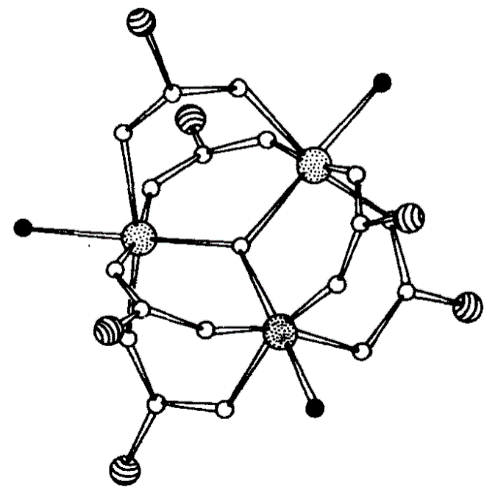
\includegraphics[scale=0.9]{M3O.png}
		\caption{三羧酸氧心配合物的结构示意图}
	\end{figure}
	\par
	同一个配合物中的三个金属离子不同,引入了结构中的非对称因素,当M=Co时,金属离子与中心氧原子的距离为1.91埃,
	与其他氧原子的距离则是2.03埃,实验数据证实了这种不对称性。量子化学计算表明,M3O骨架中,
	中心氧原子的\ce{p_z}轨道和三个金属离子的\ce{d_{xy}},\ce{d_{yz}}轨道形成四中心的d–p $\pi$键,
	增大了M-O的键级,稳定了三角形骨架结构,也使金属离子通过四中心的d–p $\pi$键互相影响。
	\subsection{配合物的合成晶体培养}
	希望利用单核金属离子的配合物(一般而言是动力学活性高,易获取的,比如水合离子)在有
	\ce{CCl_3COO^-}存在的碱性条件下水解来制备三核氧心配合物。其中溶剂的选择比较关键,
	这里选择THF与少量水的混合溶剂,反应物(尤其是金属离子)和目标产物配合物在其中有相当
	的溶解度,但是副产物NaCl并不溶于其中而是聚集在水相(产物难溶于水),这样极大地方便了后续的分离,
	同时THF也充当配体。
	\par 
	培养晶体时采用了混合溶剂,即含有少量THF的正戊烷溶液,由于正戊烷容易挥发,可以快速地
	培养出质量较好的晶体。但是由于THF是良溶剂且不易挥发(理想情况下良溶剂易挥发,不良溶剂
	不易挥发),如果在配制溶液时加入了较多THF,有可能导致晶体在溶液快挥干时大量产生,结晶效果
	不理想。
	\section{实验步骤}
	实验时间:2021年4月2日星期五\\
	\par 
	实验地点:北京大学化学与分子工程学院D区三层第二实验室2号实验台
	\subsection{配合物\ce{Fe_2MnO(OOCCCl_3)_6(THF)_3}的合成}
	\paragraph{(1)}称取2.0mmol,0.54g(0.55g)
	\footnote{括号中为实际称取的量,文中其他部分采用相同的约定}
	\ce{FeCl_3*^H_2O}与0.1mmol,0.20g(0.21g)\ce{MnCl_2*4H_2O}
	溶于5ml THF与0.5ml去离子水中,搅拌至固体溶解,记为溶液A。
	\paragraph{(2)}
	称取1.11g(1.11g)\ce{CCl_3COONa}溶于0.5ml去离子水中,记为溶液B。在此步操作中,
	实验者对于溶液的加热不够充分,导致\ce{CCl_3COONa}固体没能完全溶解,这有可能是
	后续实验出现问题的一个关键因素。
	\paragraph{(3)}
	将B溶液趁热\textbf{滴加}入A中,不断搅拌
	\footnote{这里滴加要慢,同时用磁力加热搅拌器充分搅拌,实验者在第一次实验时未使用
	滴管缓慢滴加,导致加入B溶液后局部碱性过强,铁离子发生了比较严重的水解产生了一些
	胶体物质,这对后面的晶体生长造成了较大影响。}
	,可以观察到溶液逐渐变为深红棕色,有白色糊状沉淀聚集在烧杯底部,用胶头滴管
	吸出底部沉淀。
	\paragraph{(3)}
	将烧杯中的有机溶剂在加热条件下挥干,直到溶液中只剩下红棕色固体,注意可以保留少量水分,
	如果完全干燥,容易将产物吹出。用去离子水转移固体,抽滤并用去离子水洗涤2-3次。干燥后称重,
	获得配合物\ce{m_{Mn}}=0.47g
	\footnote{理论产量为1.373g}
	,产率34\%,产物为深红棕色固体。
	在此步骤中观察到抽滤及其缓慢,个人认为是在合成时B溶液加入过快产生了部分氢氧化铁胶体
	堵住滤纸孔隙导致。
	\subsection{配合物\ce{Fe_2MnO(OOCCCl_3)_6(THF)_3}晶体培养}
	取一小勺产品,溶于3-4滴THF与5ml正戊烷的混合溶液中,搅拌溶解,过滤后装入干燥洁净的
	高型称量瓶中。配置两份溶液,一份置于开启通风的通风橱中,一份置于未开启通风的通风橱中。
	静置等待结晶。可能是由于溶液中又有部分胶体,结晶过程并不顺利,最后没能观察到有着晶体
	外形的沉淀物,只观察到了圆片状的固体,如图:
	\begin{figure}[htbp]
		\centering
		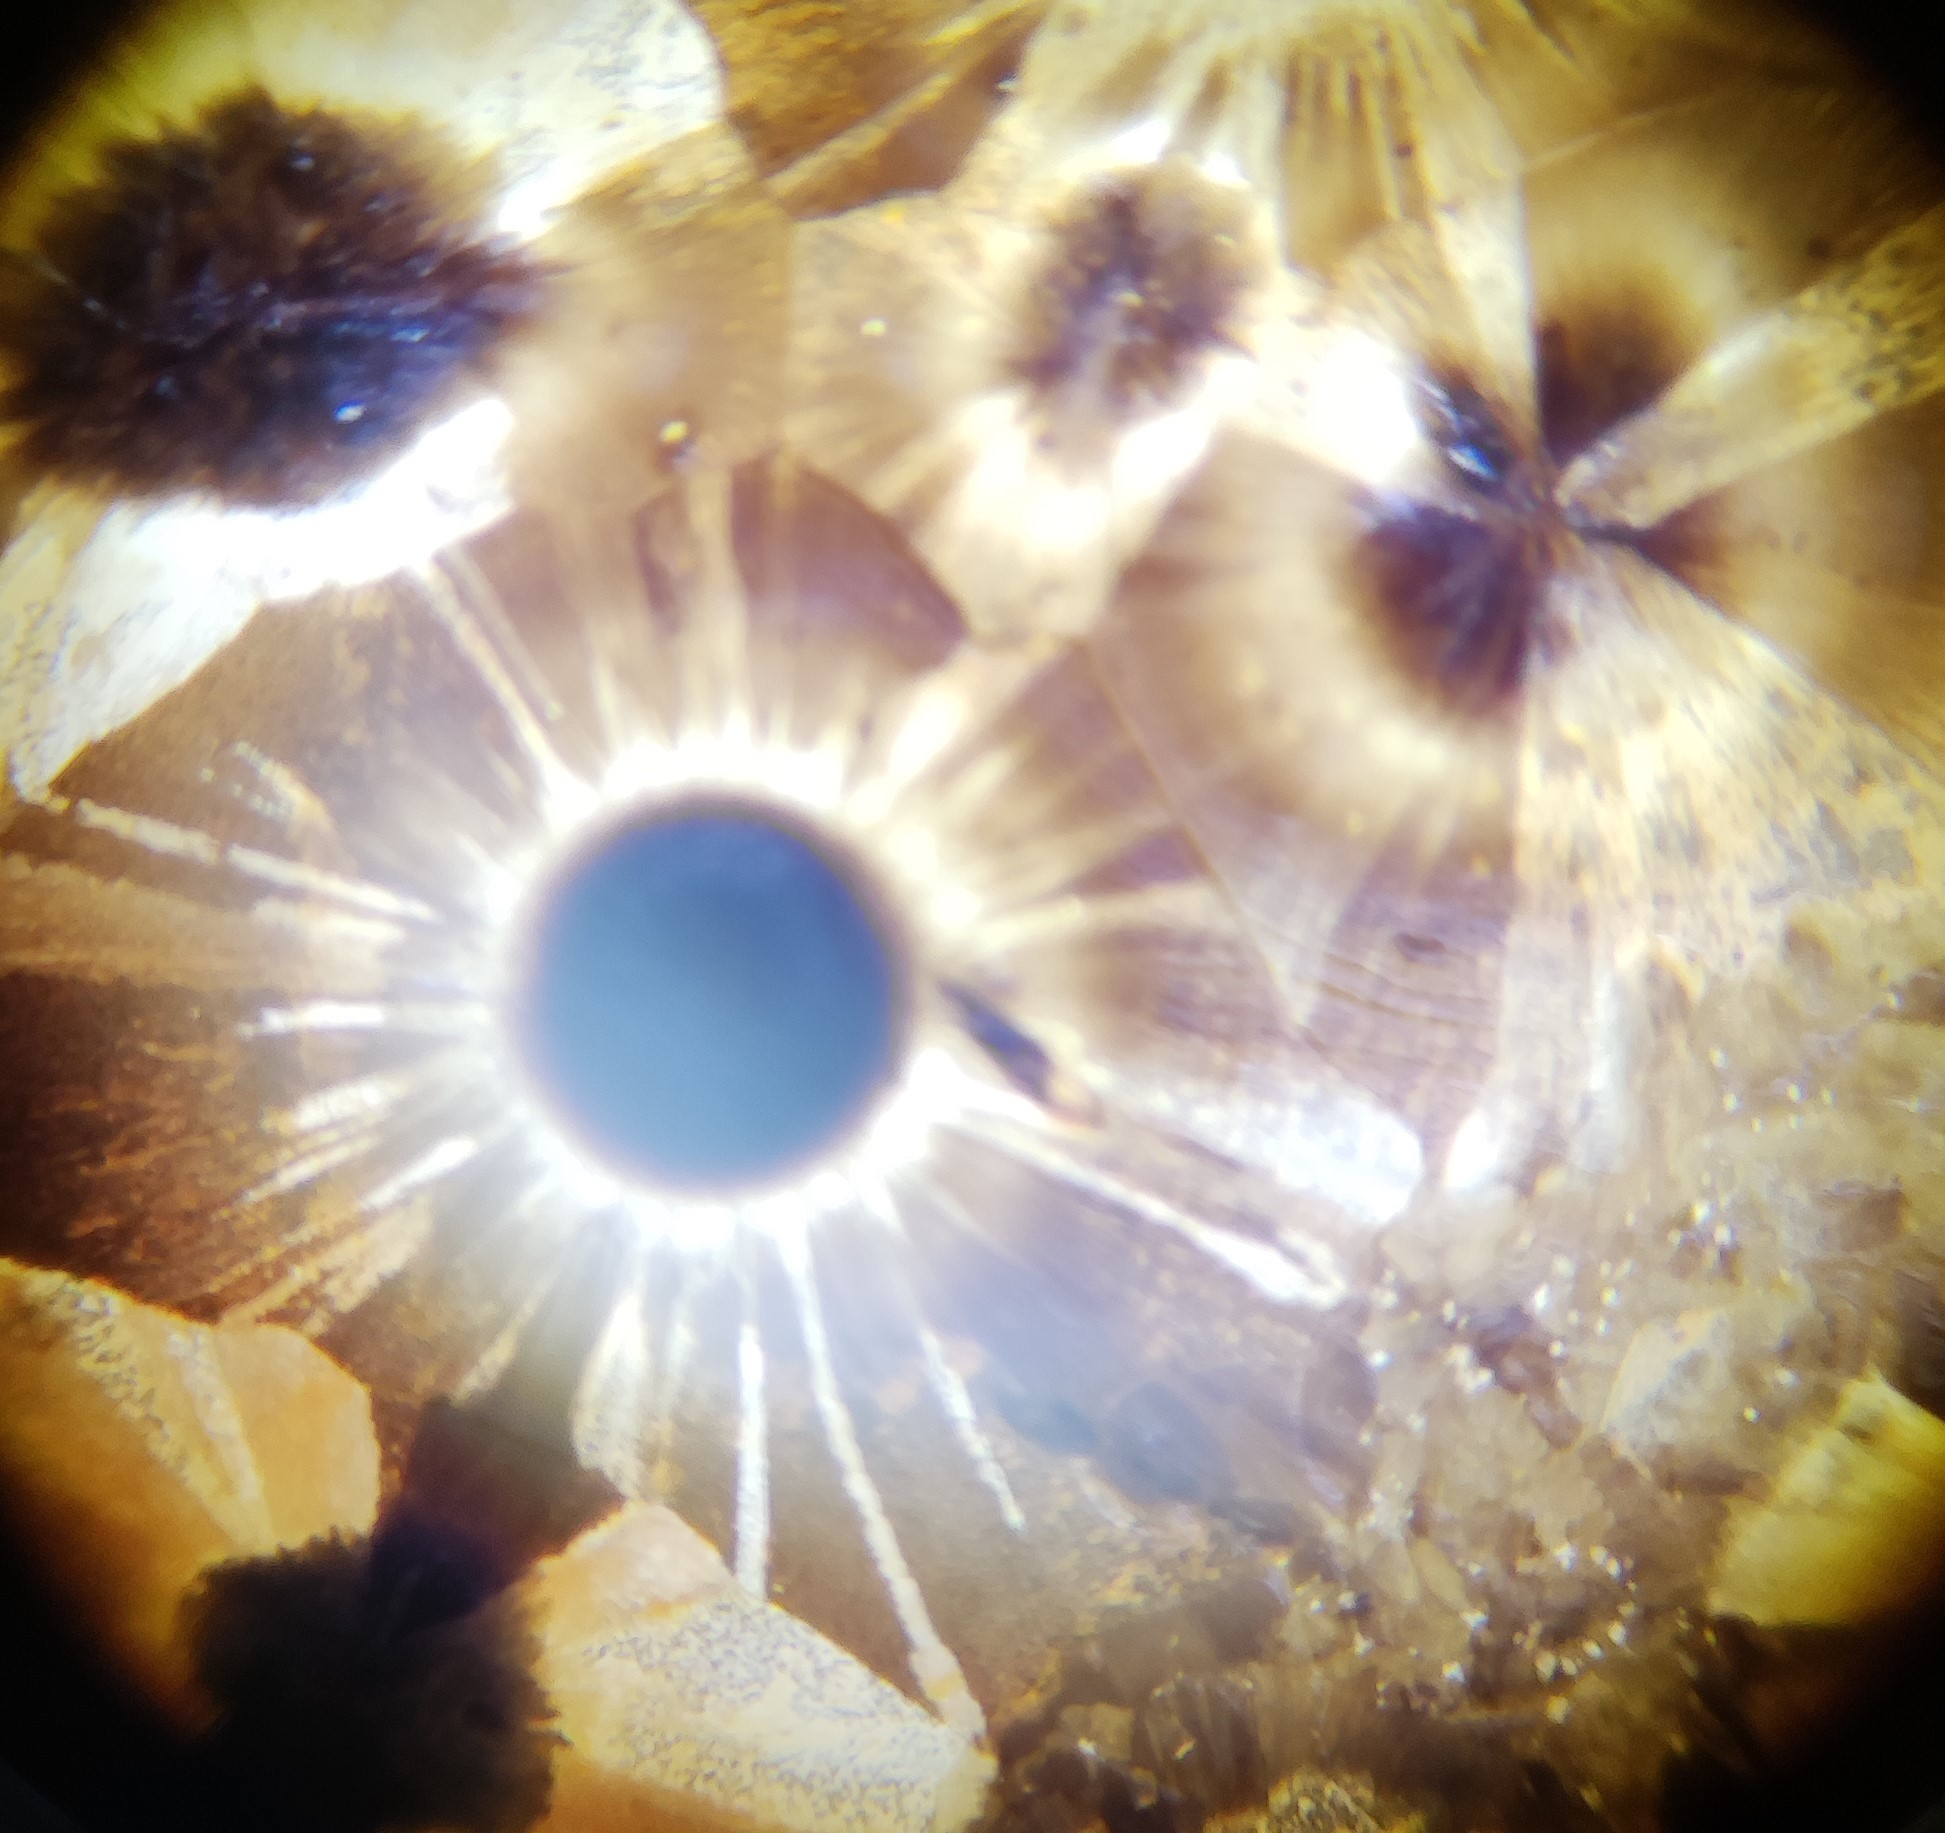
\includegraphics[scale=0.1]{Mn_WCB.jpg}
		\caption{含锰配合物的“晶体”照片}
	\end{figure}
	\par 
	同时可以观察一下结晶较好的同学的晶体:
	\begin{figure}[htbp]
		\centering
		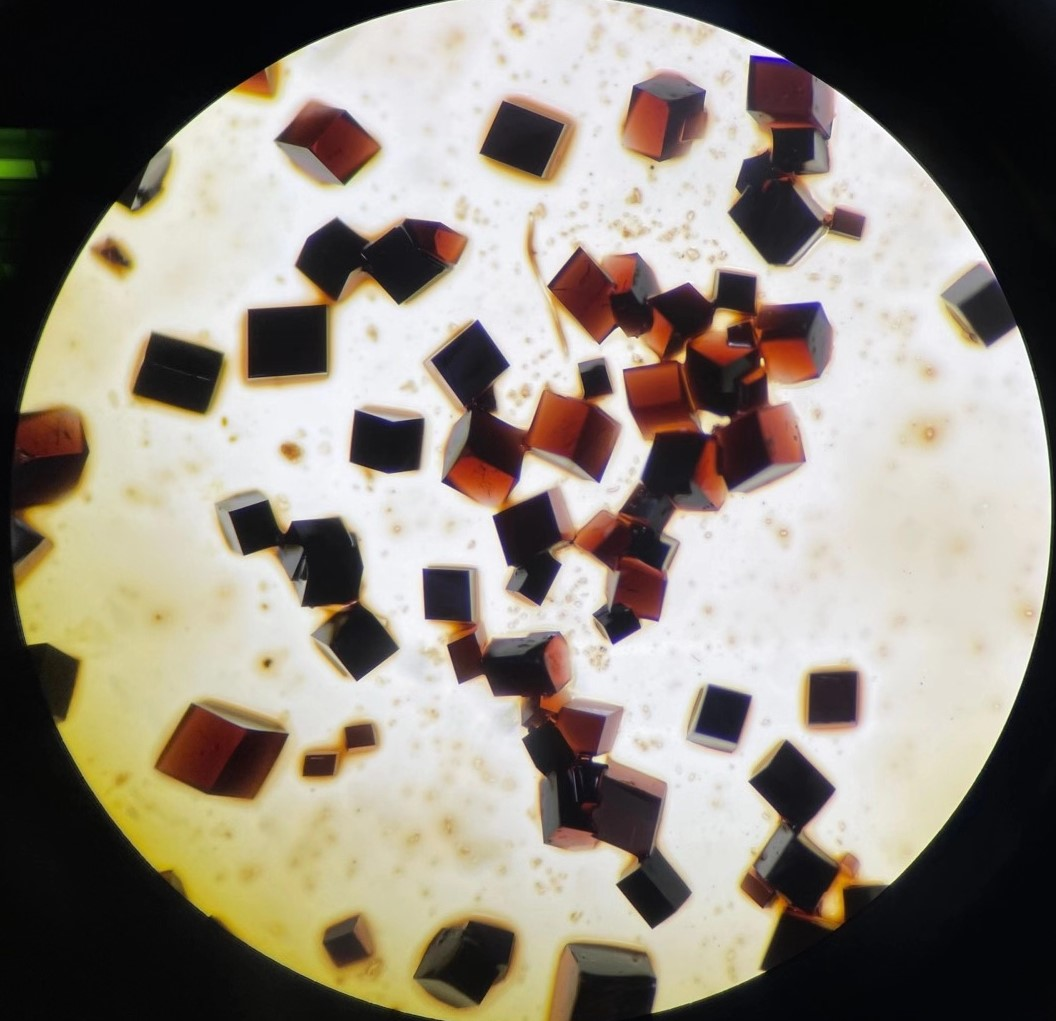
\includegraphics[scale=0.30]{Mn_LXY.jpg}
		\caption{含锰配合物的晶体照片by LXY}
	\end{figure}
	可以看到晶体呈现出棕色,棱角分明,从晶体顶点的角度可看出大部分晶体具有3重旋转对称性
	,其有可能属于三方晶系。
	\subsection{配合物\ce{Fe_2NiO(OOCCCl_3)_6(THF)_3}的合成}
	\paragraph{(1)}称取2.0mmol,0.54g(0.54g)
	\ce{FeCl_3*^H_2O}与0.1mmol,0.24g(0.25g)\ce{NiCl_2*6H_2O}
	溶于5ml THF与0.5ml去离子水中,搅拌至固体溶解,记为溶液A。
	\paragraph{(2)}
	称取1.11g(1.11g)\ce{CCl_3COONa}溶于0.5ml去离子水中,记为溶液B。在此步操作中,
	实验者充分加热溶解了\ce{CCl_3COONa},避免了上一步出现的失误。
	\paragraph{(3)}
	将B溶液趁热\textbf{滴加}入A中,不断搅拌
	,可以观察到溶液逐渐变为棕黄色,有白色糊状沉淀聚集在烧杯底部,为了避免氢氧化物
	出现在产物中,这次实验者改用胶头滴管将上清液吸出。
	\paragraph{(3)}
	将烧杯中的有机溶剂在加热条件下挥干,直到溶液中只剩下棕黄色固体。用去离子水转移固体,抽滤并用去离子水洗涤2-3次。干燥后称重,
	获得配合物\ce{m_{Ni}}=0.33g
	\footnote{理论产量为1.373g}
	,产率24\%,产物为棕黄色固体,产率较低有可能是因为在转移上清液的过程中损失了比较多的产物。
	\subsection{配合物\ce{Fe_2NiO(OOCCCl_3)_6(THF)_3}的晶体培养}
	培养过程与之前完全一致,不过由于时间限制,只尝试了没有开通风橱的情况。
	\begin{figure}[htbp]
		\centering
		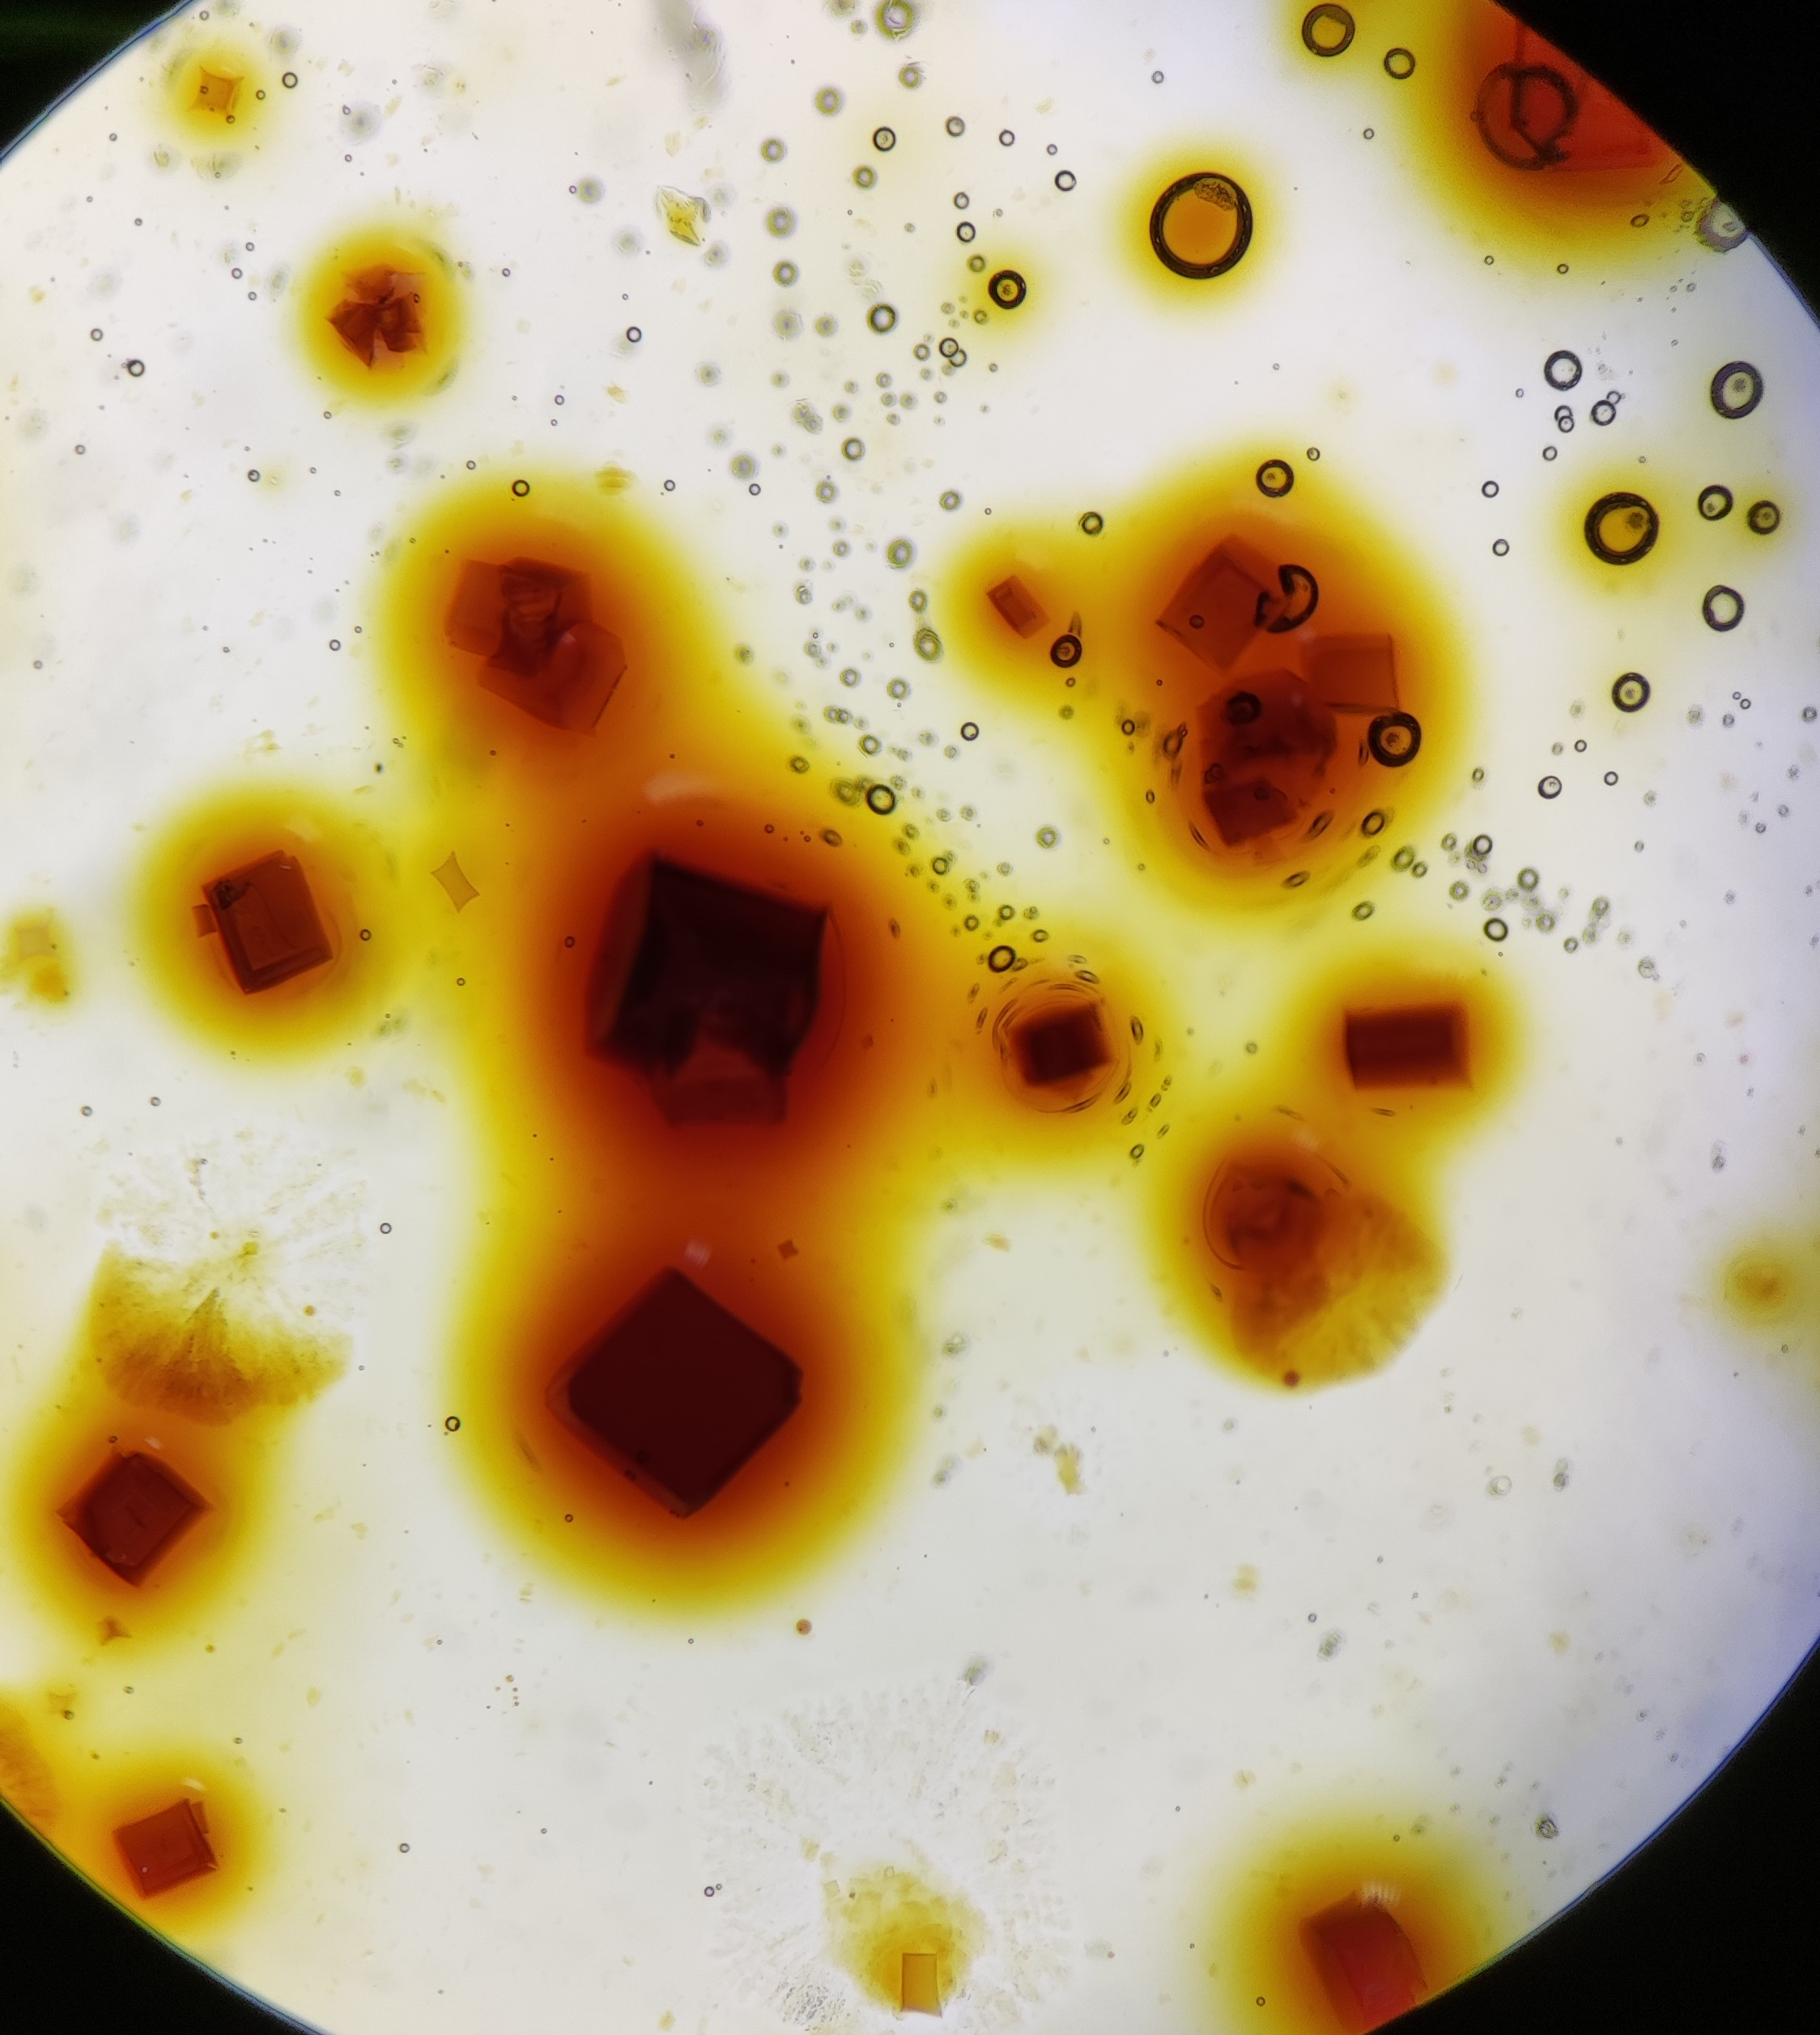
\includegraphics[scale=0.1]{Ni_WCB.jpg}
		\caption{含镍配合物的晶体照片}
	\end{figure}
	可以从图中看出,晶体表面平面之间的夹角趋近于90\degree ,与真实的晶胞参数($\alpha = \beta = \gamma = 84.12^\circ$)
	非常接近,可以认为这个晶体是沿着[100]面生长的。
	\section{结果与讨论}
	\subsection{配合物的吸收光谱}
	\paragraph{(1)}称取0.15g产品溶于5ml THF中,测定700-1100nm波段的吸收光谱,小组内
	三种不同金属配合物的吸收光谱如下图所示(其中Mn为本人的样品)。
	\begin{figure}[htbp]
		\centering
		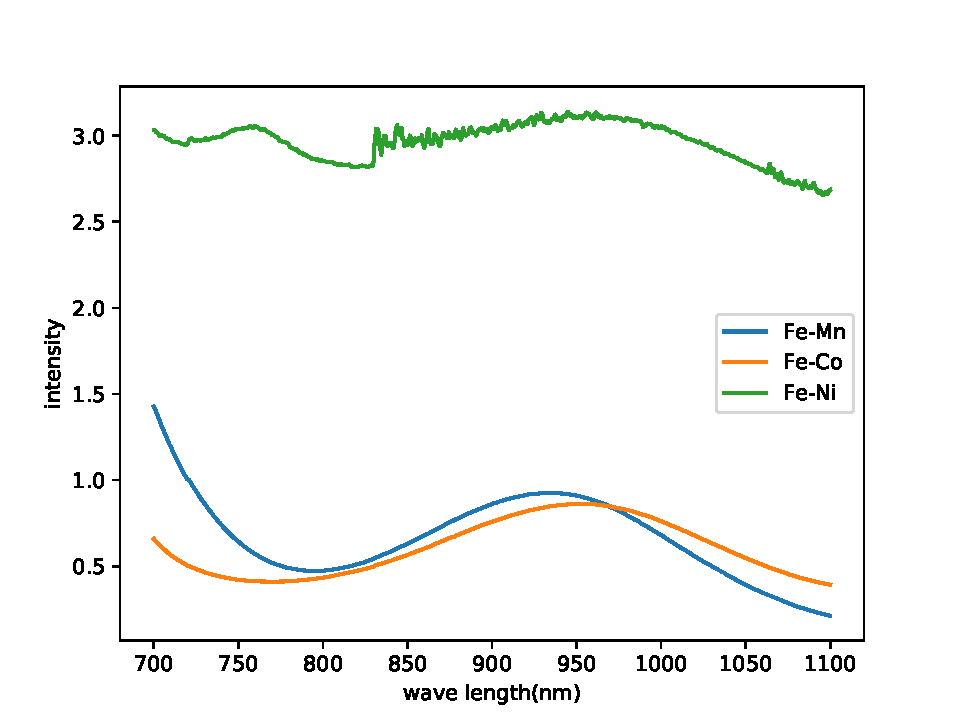
\includegraphics[scale=0.65]{compare.pdf}
		\caption{实验合成出的三种含有不同金属的三核配合物的吸收光谱}
	\end{figure}
	能够明显地看到含镍的配合物样品吸收曲线明显与另外两个有区别:吸收曲线不平滑、摩尔吸光
	系数明显偏大。这并不是因为镍与其他两种金属的区别造成的,而是溶液中有比较多的胶体、
	对光有比较强的散射造成的。通过查看原始数据,可以得到Mn吸收峰的位置为:934nm,强度为0.925,
	可以计算出摩尔吸光系数为(假设盛装样品的比色皿长度为1cm):42\ce{L*mol^{-1}cm^{-1}};
	Co吸收峰的位置为:948nm,强度为:0.860, 摩尔吸光系数为:39\ce{L*mol^{-1}cm^{-1}}。
	\par 
	能够看出从\ce{Mn\to Co}吸收峰的波长由短变长,说明\ce{^6A_1\to ^4T_1}的能级差减小,
	考虑到\ce{d^5}构型的Tanabe-Sugano图:
	\begin{figure}[htbp]
		\centering
		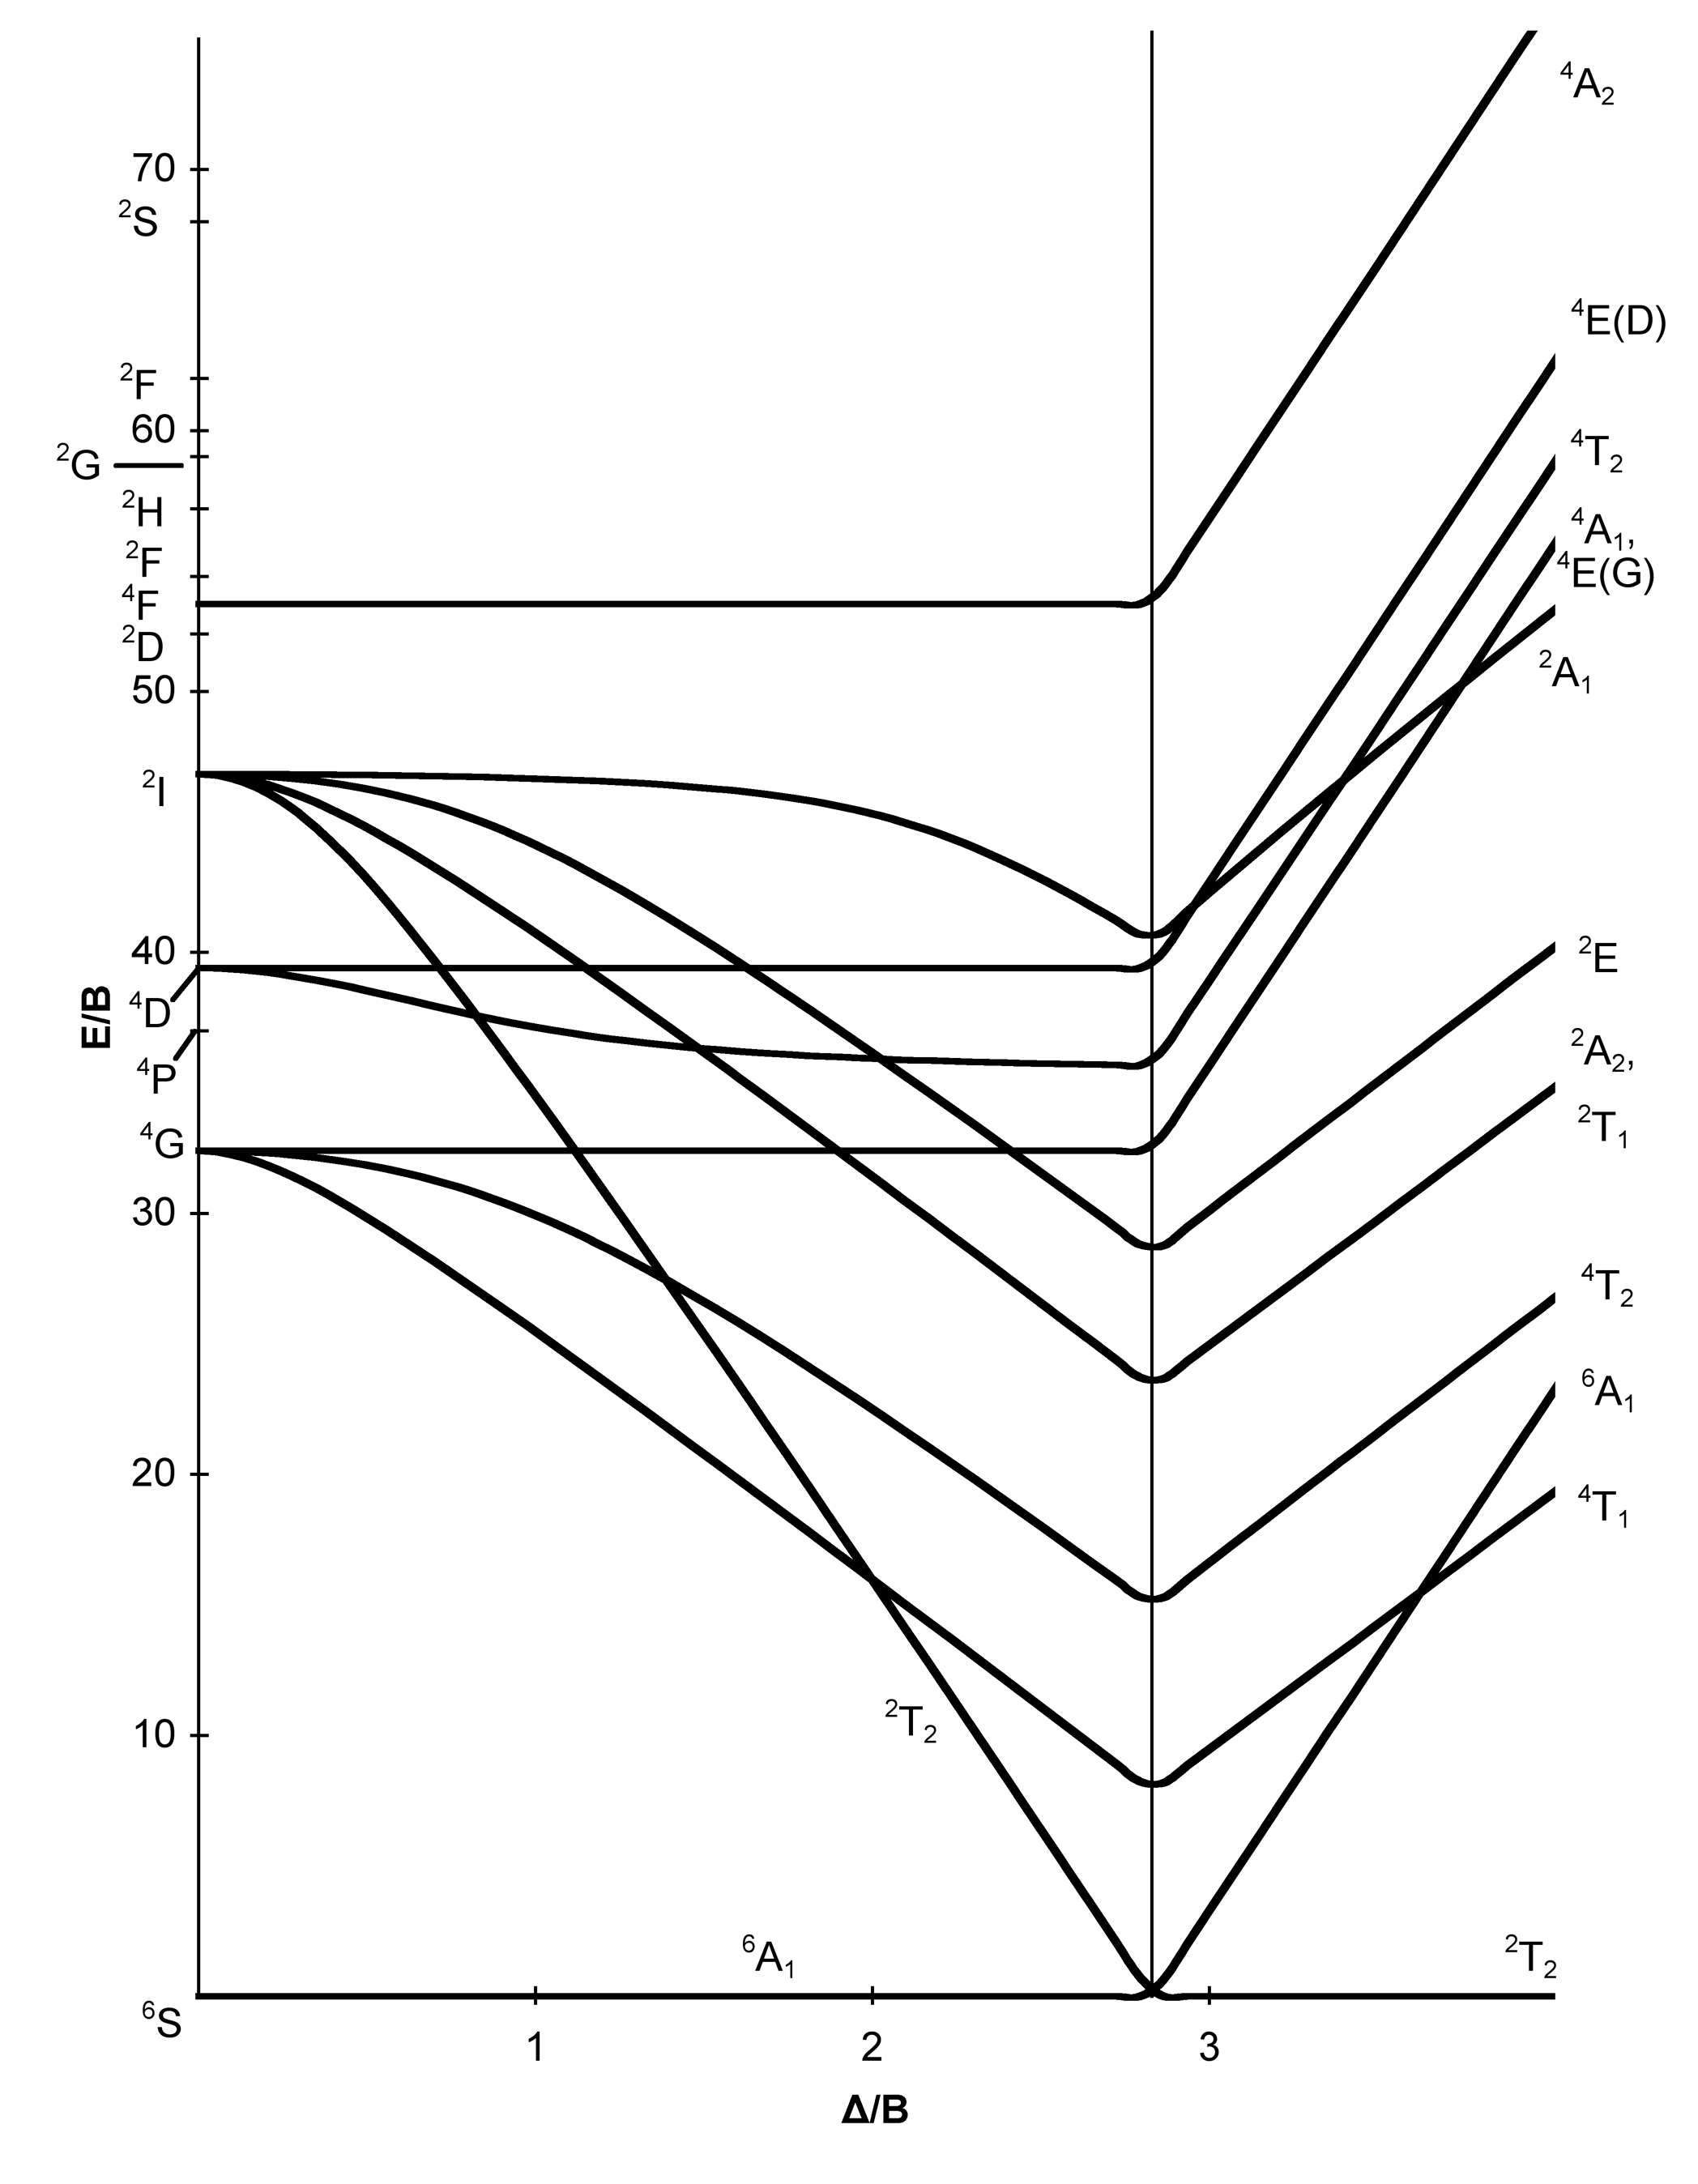
\includegraphics[scale=0.10]{D5_Tanabe-Sugano_diagram.png}
		\caption{\ce{d^5}构型的Tanabe-Sugano图}
	\end{figure}
	可以看到在高自旋状态下,这两个能级之间的能量差随着配位场的增强而下降,这说明
	从\ce{Mn\to Co},其配位场是不断增强的。由于\ce{Fe^{3+}}周围的配位环境没有发生变化,
	因此能使配位场增强的因素只有减小配体与中心原子之间的距离,这一点可以从Mn晶体的晶胞体积
	(a = 13.715埃)
	比Co晶体(a=13.671埃)的大得到验证,至于这种体积的缩小,很有可能与\ce{Co^{2+}}的半径比
	\ce{Mn^{2+}}更小有关,这导致整个配合物的结构更加紧凑。
	\subsection{如何获得更高质量的晶体}
	本实验探究了在不同条件晶体的生长情况,由于本人的晶体没有长成功,这里借用一下
	喻琪锐同学的照片:
	\begin{figure}[htbp]
		\centering
		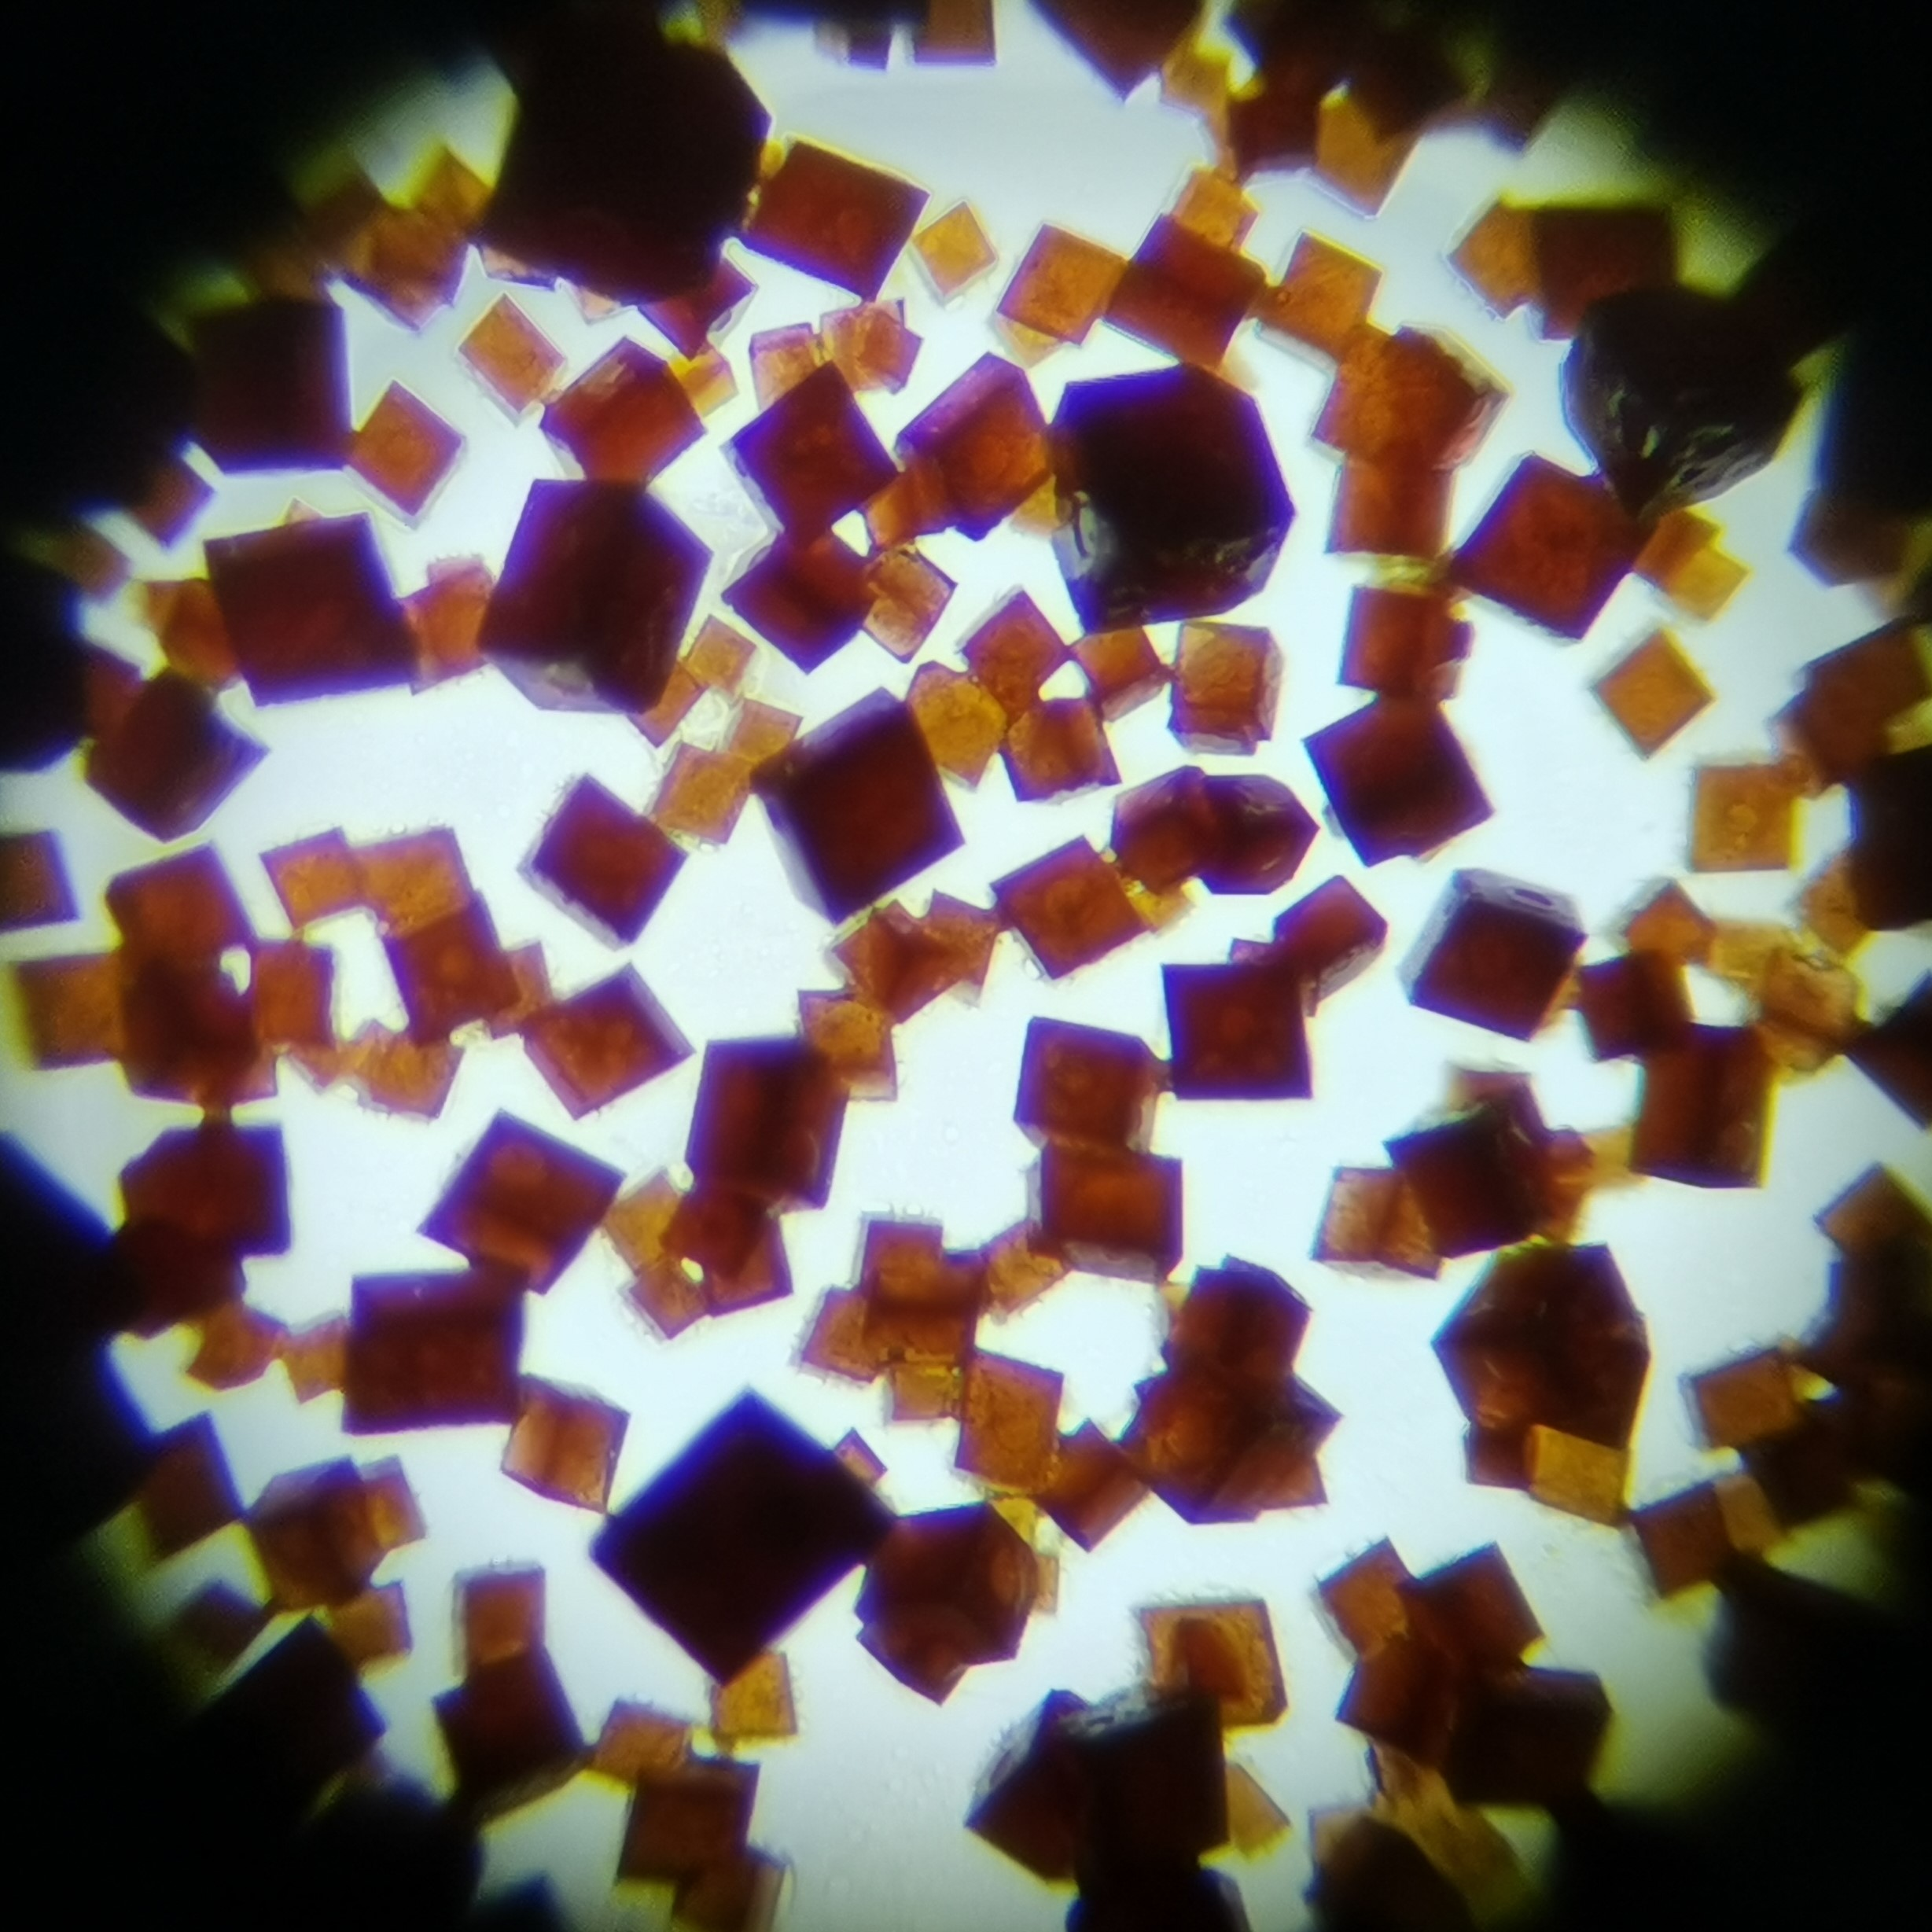
\includegraphics[scale=0.10]{Ni_YQR_T.jpg}
		\caption{含镍配合物在溶液被晃动过后的晶体生长}
	\end{figure}
	\begin{figure}[htbp]
		\centering
		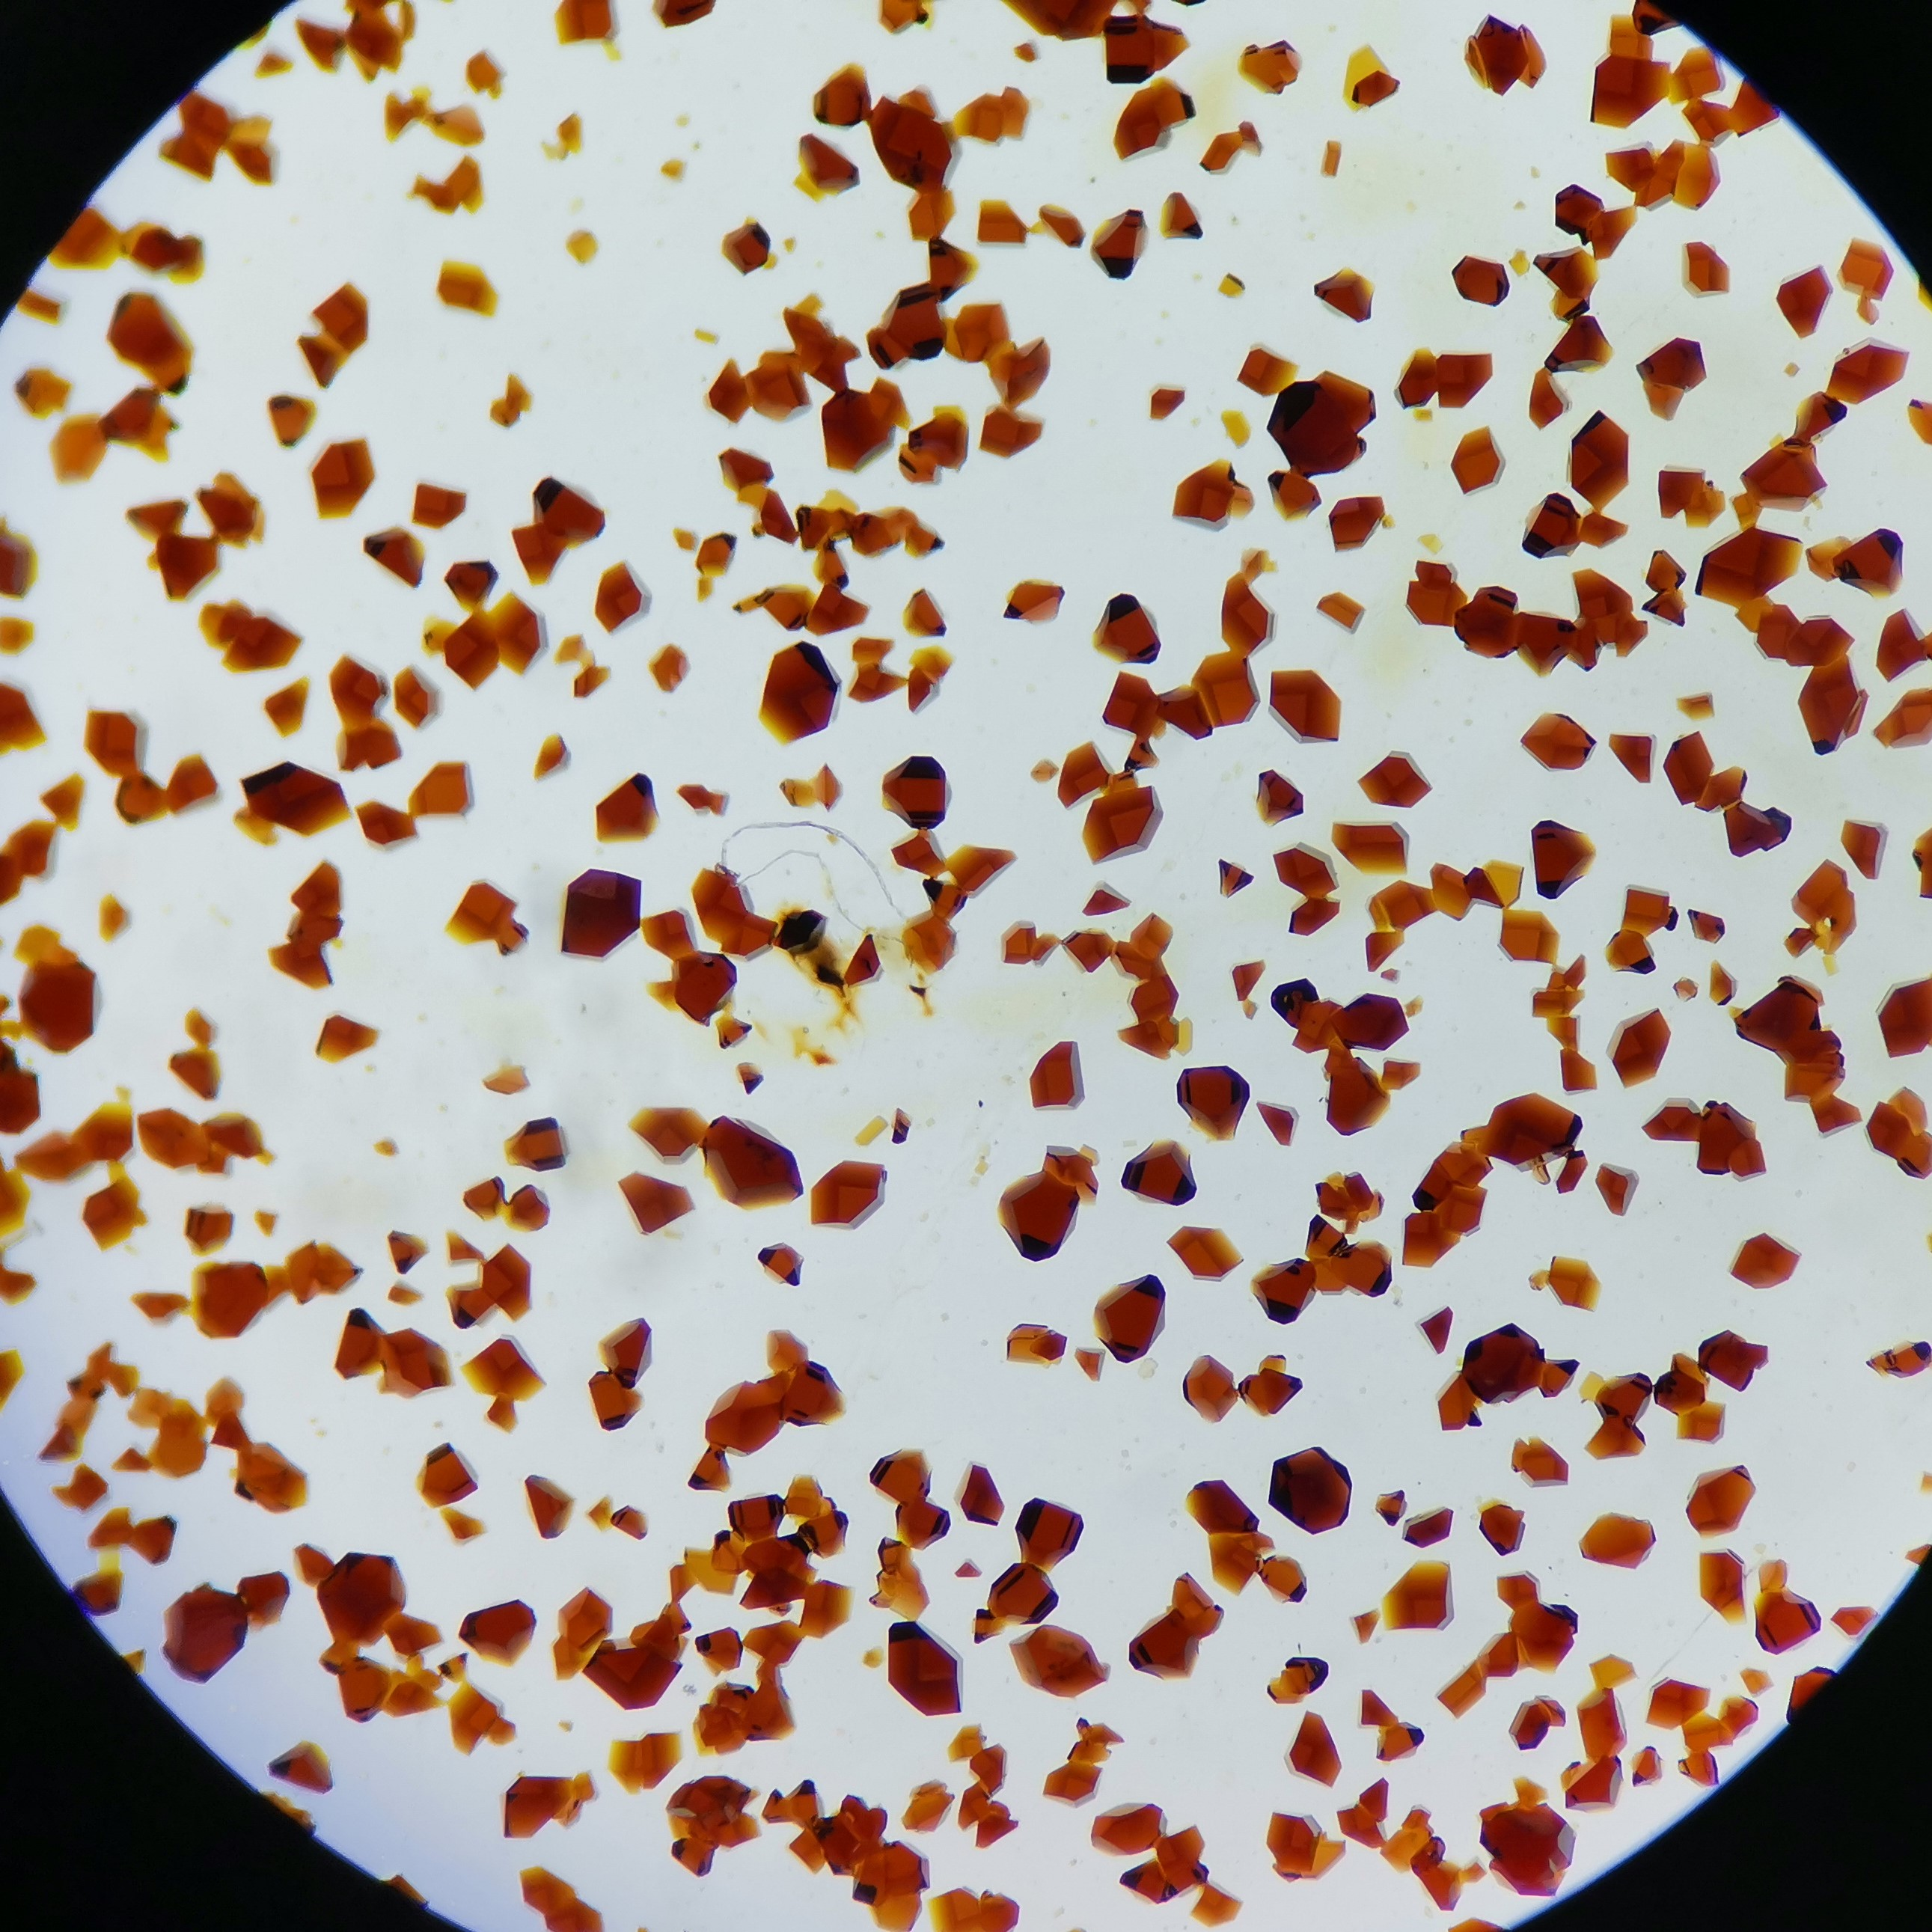
\includegraphics[scale=0.10]{Ni_YQR_N.jpg}
		\caption{含镍配合物在溶液静置的晶体生长}
	\end{figure}
	可以看到,晃动溶液会使得晶体数量变多、体积变小,这是由于晃动过程会破坏原有晶体的生长
	,同时创造更多的结晶中心。
	\bibliographystyle{plain}
	\bibliography{ref}
\end{document}